\section{$B$ meson production in proton-proton collisions}

A proton-proton collision ($pp$-collision) is the interaction between two high energetic protons through the strong force.
The exchange of gluons between those protons initiates the production of multiple particles. 
A dominant process is the fusion of two gluons into one gluon, which then decays into a quark-antiquark pair.
These quarks then form hadrons by combining with quarks that emerge from the vacuum in pairs.
This process is called hadronization and further produces fragmentation particles through the hadronization of the emerging unpaired quarks.

At LHCb, a frequent goal is to analyse $B$ meson candidates in $pp$ collisions, often called the signal $B$.
$B$ mesons are composed of one $b$~quark and one of the $u/d/c/s$ quarks and have a mean life time of $\unit{\pico\second}$.
When the $b$ quark is the decay product of the fused gluon in a $pp$ collision, the signal $B$ is Lorentz boosted.
This allows the distinction of the production point and the decay point of the signal $B$.
Relevant for this thesis are the uncharged $B$~mesons
\begin{align*}
    B^0 &= \bar{b}d \, , & \bar{B}^0 &= b\bar{d} \, , & B_s^0 &= \bar{b}s \, , & \bar{B}_s^0 &= b\bar{s} \, .
\end{align*}

Analysing the signal $B$ can be done by reconstructing the signal decay or by reconstructing the associated event. 
The latter method is independent of the signal decay channel, and it is often used in flavour tagging algorithms at LHCb. 
A similar method is used in this thesis.
An example schematic of a proton-proton collision is shown in \autoref{fig:ft_scheme}. 
This schematic excludes particles which are unassociated with the signal $B$ that are contained in the underlying event.

\begin{figure}
    \centering
    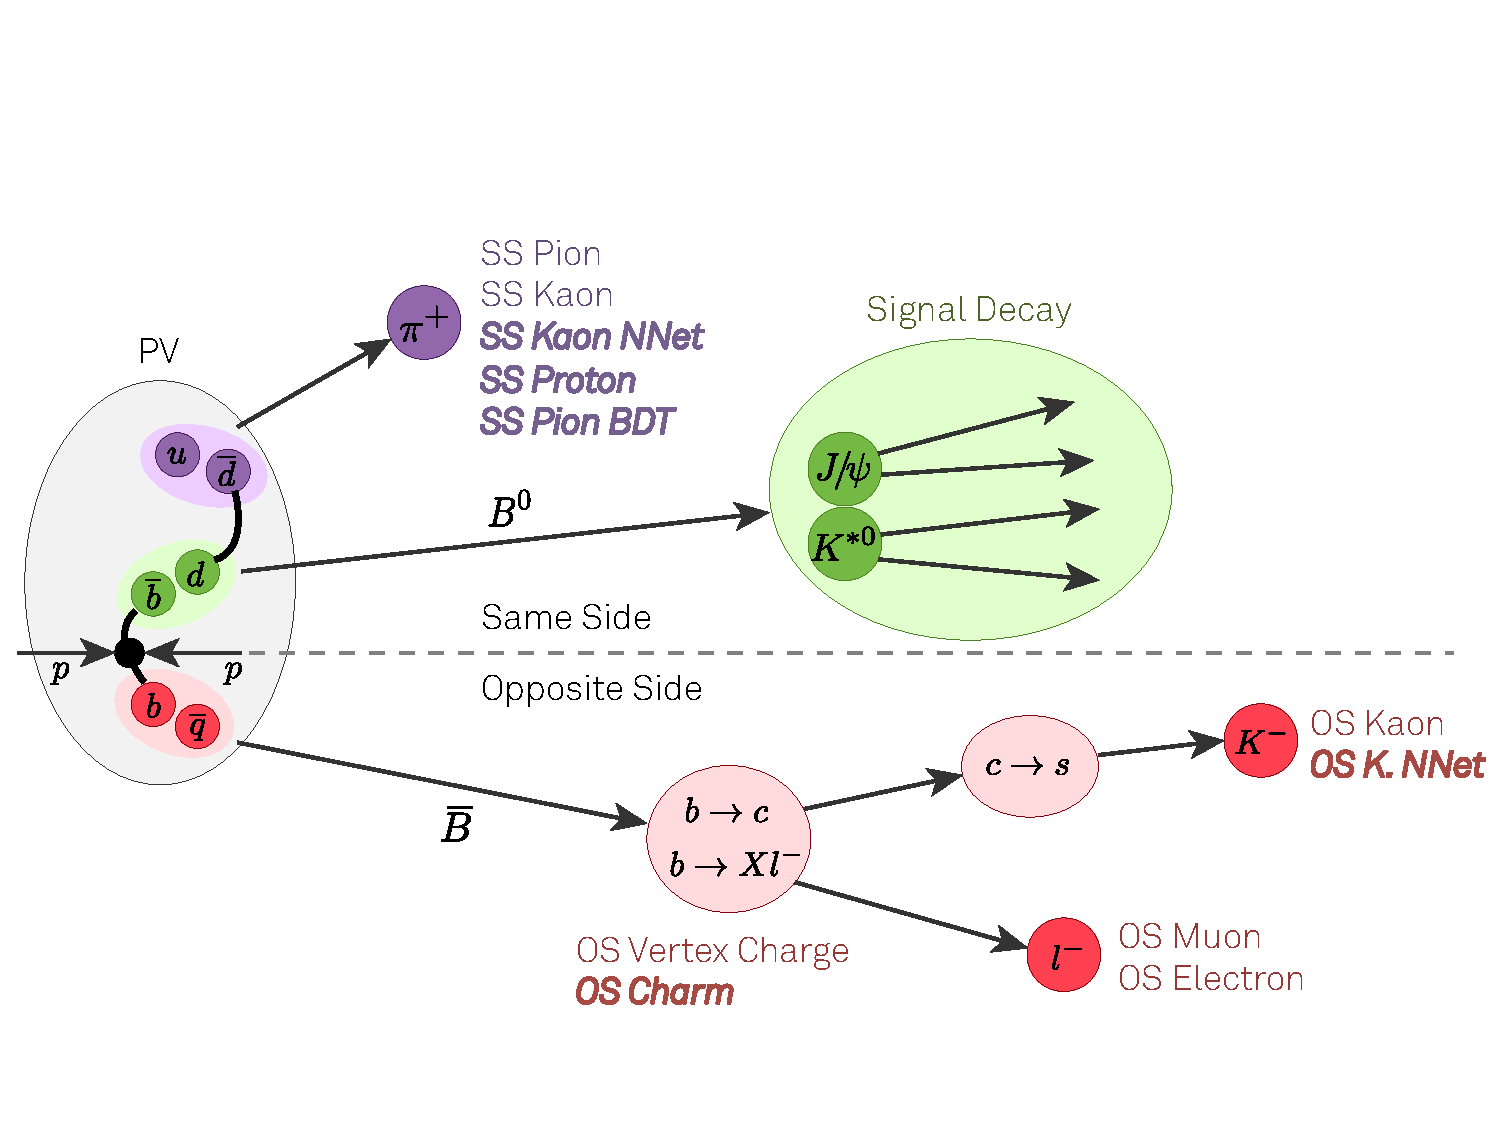
\includegraphics[width=\textwidth]{images/FlavourTaggingScheme.pdf}
    \caption{Schematic overview of the underlying principles of LHCb's flavour tagging algorithms \cite{ft_scheme}.}
    \label{fig:ft_scheme}
\end{figure}

The collision point of a $pp$ pair is called the primary vertex~(PV), and the decay point of the signal $B$ is called the secondary vertex~(SV).
The back-to-back production of the $b\bar{b}$ pair leads to a separation of the associated event.
The same side~(SS) contains the decay particles and the fragmentation particles of the signal $B$.
The opposite side~(OS) contains all particles associated with the $b$ quark not in the signal $B$.
To identify the signal $B$ it is sufficient to use information about either the SS fragmentation, the signal decay or the OS.
